\section{Semi-automated tracking.}

Let us suppose we are dealing with a difficult image in which me must track only a subset of cells. 
The cells are difficult to track automatically, for instance because there are many spurious structures labelled. 
Or because there are other cells of different sizes in the tissue we are studying. 
Or because the image quality varies in time and space. 
The data is such that that fully automated algorithms introduced in chapter~\ref{Getting_started} won't give us fully accurate results. 
We can use the manual editing tools introduced in chapter~\ref{Manuel_Editing} and curate the results of automated tracking, removing spurious detections and links, and fixing incorrect ones. 
Another approach would be to start from a blank annotation and track manually only the cells we are interested in. 
Both approaches might be long and tedious. 
We introduce in this chapter tools for semi-automated tracking, that should alleviate the work of the second approach.

Semi-automated tracking is simply a way of following a specific cell that you picked-up manually. 
The tracker will follow the cell over time, and create spots and links for a certain amount of time-points.
It searches for the best location candidate in the next time-point around the location of the spot.
It then creates a new spot there and links it to the previous one.
This procedure is repeated this for a certain number of time-points you can set, creating or augmenting a track starting from the spot you selected.

The semi-auto tracker can be configured to work backward in time (backtracking), to have a certain search radius, or a certain sensitivity to spot quality (as defined in chapter~\ref{Detecting_Cells}).
The way it interacts with existing annotation can be configured too. 
You can make it stops when it meets an existing spot, linking to it or not.
You can make it connect to small tracks and resume tracking when it meets the track end.
You can force it to only create links on already existing spots. 
These configuration options give rise to several use-cases we will also survey in this chapter.
But the important message is that semi-automated tracking is a convenient means for dealing with difficult cases, when a fully automated approach fails, and when the data to track is large that doing it manually is inconvenient.

\subsection{Simple semi-automated tracking.}

We will introduce semi-automated tracking on a movie with empty annotation. 
Open the dataset we have been using so far, and clear all annotations (for instance select all \keys{\ctrl+A} then delete selection \keys{\shift+\backdel}).
Then pick a cell in the top layer, and create a spot, centered on its brightest part, like for instance on Figure~\ref{fig:BeforeSemiAutoTracking}.
Adjust its radius and select it.

\begin{figure}
    \centering
    \null\hfill
    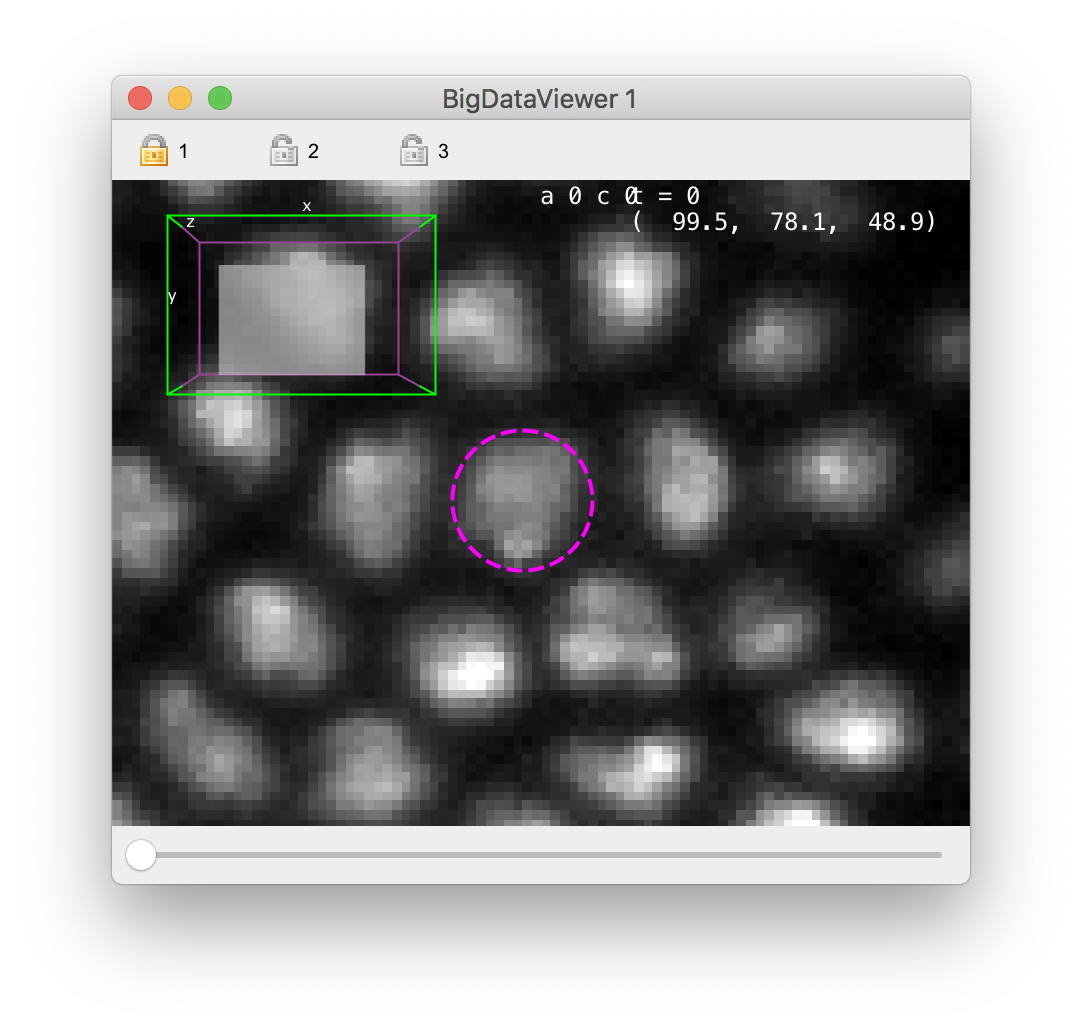
\includegraphics[width=0.3\textwidth]{figures/Mastodon_SemiAutoTracking_01a.png}
    \hfill
    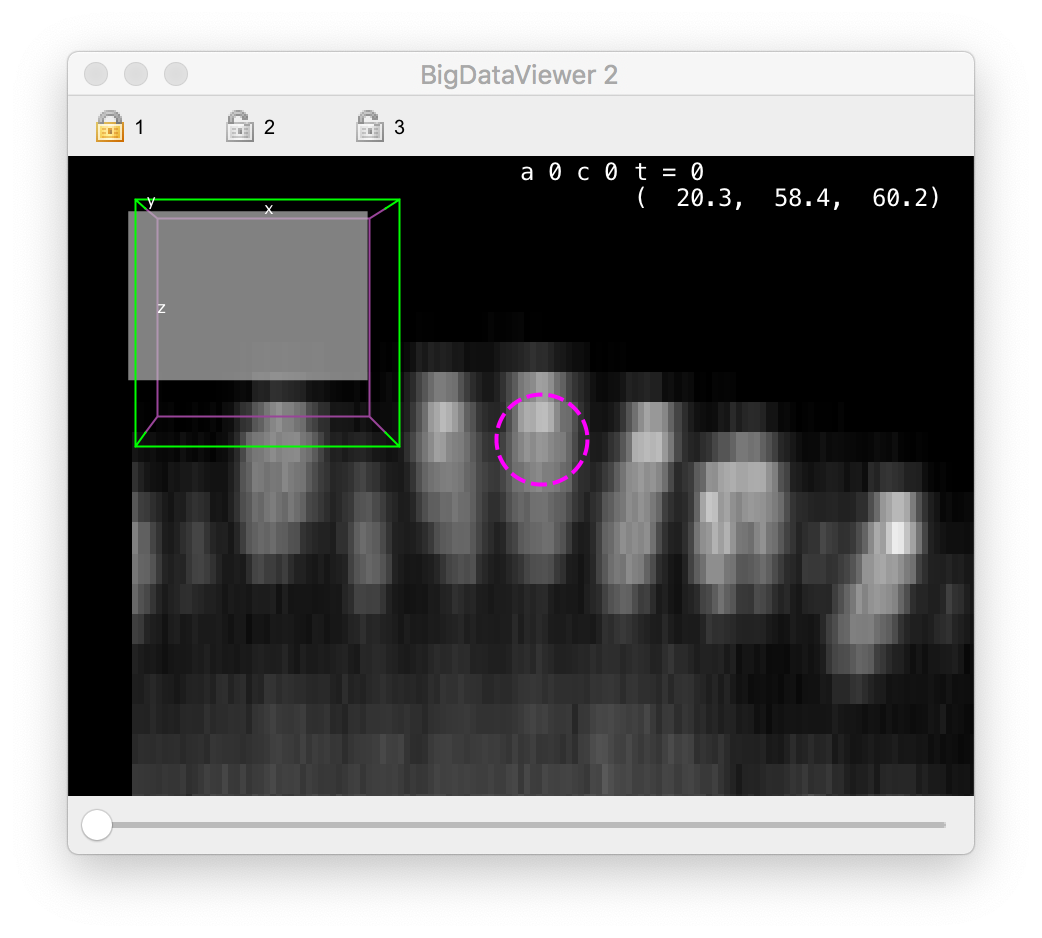
\includegraphics[width=0.3\textwidth]{figures/Mastodon_SemiAutoTracking_01b.png}
    \hfill\null
    \caption{Manually picking a cell for semi-automated tracking.}
    \label{fig:BeforeSemiAutoTracking}
\end{figure}

To start semi-automated tracking, press \keys{\ctrl+T}.
A log window should open, and tracking should proceed. 
If the log does not complain about candidates being too far, you should end up with something resembling Figure~\ref{fig:AfterSemiAutoTracking}.
The tracking stopped after 10 frames, and the last spot added is now in the selection. 
Each spot is centered on the cell we started with, and it has the same radius that of the first spot we created. 
You can resume semi-automated tracking from the last spot created by just pressing \keys{\ctrl+T} again. 
If you do it one more time you should reach the end of the movie, with a new track following a single cell over the full movie duration.
To get it, you just had to press \keys{\ctrl+T} 3 times.

\begin{figure}
    \centering
    \null\hfill
    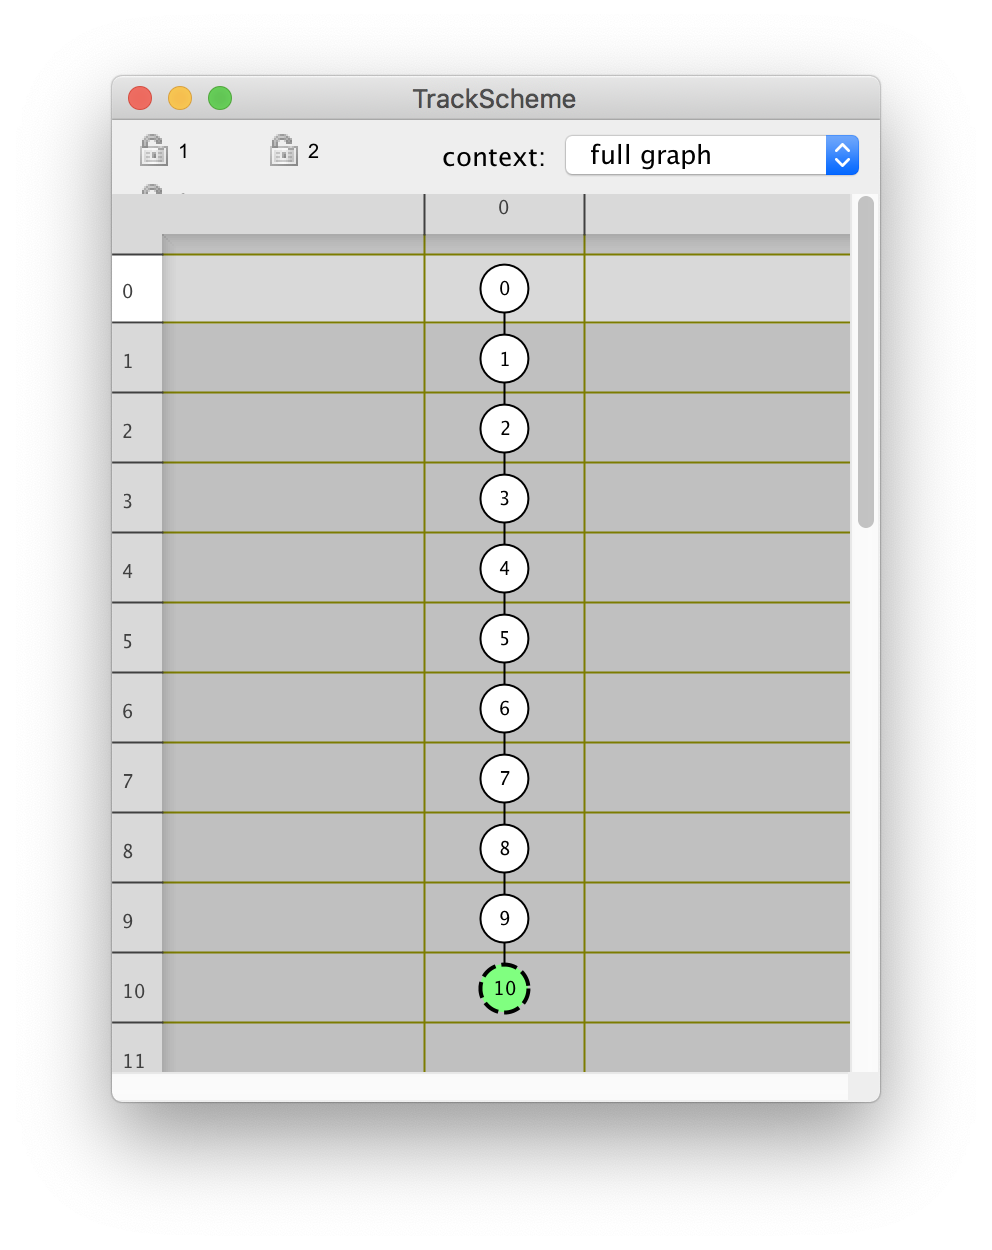
\includegraphics[width=0.2\textwidth]{figures/Mastodon_SemiAutoTracking_02.png}
    \hfill
    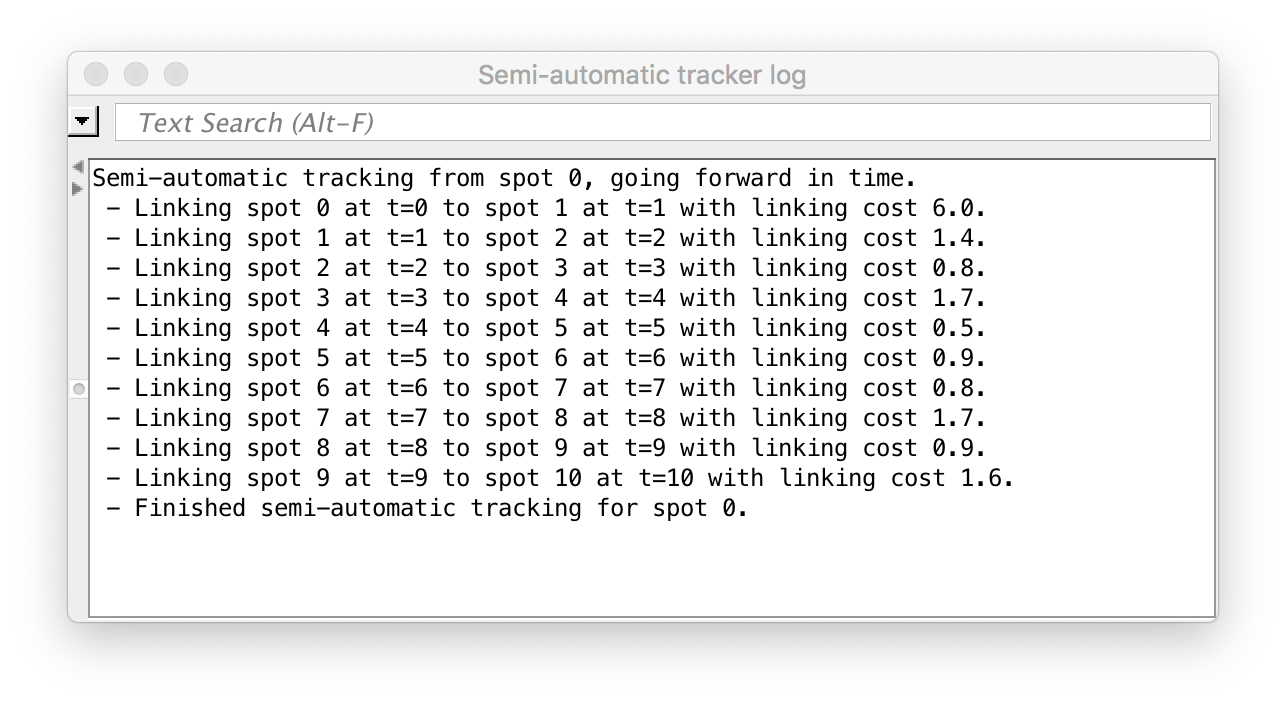
\includegraphics[width=0.4\textwidth]{figures/Mastodon_SemiAutoTracking_03.png}
    \hfill\null
    \caption{Results of semi-automated tracking.}
    \label{fig:AfterSemiAutoTracking}
\end{figure}



\subsection{Configuring the semi-automated tracker.}

\subsection{Main use-cases for semi-automated tracking.}

\subsubsection{Tracking from a blank annotation. }

\subsubsection{Patching small track segments.}

\subsubsection{Backtracking, branching on cell divisions. }

\subsubsection{Sparse linking over dense spots.}
